%  !TeX  root  =  user_guide.tex

\chapter{Компоновщик карты}\label{label_printcomposer}

% when the revision of a section has been finalized,
% comment out the following line:
% \updatedisclaimer

Компоновщик карты обеспечивает широкие возможности для подготовки макета
и печати. Он позволяет добавлять такие элементы как: карта QGIS, легенда,
масштабная линейка, изображения, фигуры, стрелки и текстовые блоки. При
создании макета доступно изменение размеров, группировка, выравнивание и
изменение положения каждого элемента, а также настройка их свойств.
Готовый макет можно распечатать или экспортировать в изображение,
Postscript, PDF или SVG формат\footnote{Экспорт в SVG поддерживается,
но может работать не корректно с некоторыми последними версиями QT4.
Необходимо самостоятельно проверить это на своей системе}, кроме того,
макет можно сохранить как шаблон и использовать его повторно в другой
сессии. Полный перечень инструментов Компоновщика приведен в
таблице~\ref{tab:printcomposer_tools}:

\begin{table}[h]\index{Print composer!tools}
\centering\small
\renewcommand{\arraystretch}{2}
 \begin{tabular}{|m{1cm}|m{5.4cm}|m{1cm}|m{5.4cm}|}
 \hline \textbf{Иконка} & \textbf{Описание} & \textbf{Иконка} &
 \textbf{Описание} \\
 \hline 
\includegraphics[width=0.7cm]{mActionFolder}
 & Загрузить из шаблона &
 
\includegraphics[width=0.7cm]{mActionFileSaveAs} & Сохранить как шаблон \\
 \hline 
\includegraphics[width=0.7cm]{mActionExportMapServer}
 & Экспорт в изображение &
 
\includegraphics[width=0.7cm]{mActionSaveAsPDF} & Экспорт в PDF \\
 \hline 
\includegraphics[width=0.7cm]{mActionSaveAsSVG} & Экспорт в SVG
 & 
\includegraphics[width=0.7cm]{mActionFilePrint}
 & Печать \\
 \hline 
\includegraphics[width=0.7cm]{mActionZoomFullExtent} & Полный
 охват & 
\includegraphics[width=0.7cm]{mActionZoomIn} & Увеличить \\
 \hline 
\includegraphics[width=0.7cm]{mActionZoomOut} & Уменьшить&
 
\includegraphics[width=0.7cm]{mActionDraw} & Обновить \\
 \hline 
\includegraphics[width=0.7cm]{mActionAddMap} & Добавить
 карту & 
\includegraphics[width=0.7cm]{mActionSaveMapAsImage}
 & Добавить изображение \\
 \hline 
\includegraphics[width=0.7cm]{mActionLabel} & Добавить текст
 composition & 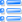
\includegraphics[width=0.7cm]{mActionAddLegend} & Добавить
 легенду \\
 \hline 
\includegraphics[width=0.7cm]{mActionScaleBar} & Добавить
 масштабную линейку & 
\includegraphics[width=0.7cm]{mActionAddBasicShape}
 & Добавить фигуру \\
 \hline 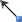
\includegraphics[width=0.7cm]{mActionAddArrow} & Добавить
 стрелку & 
\includegraphics[width=0.7cm]{mActionOpenTable} & Добавить
 таблицу \\
 \hline 
\includegraphics[width=0.7cm]{mActionSelectPan} & Выбрать/переместить
 элемент &
 
\includegraphics[width=0.7cm]{mActionMoveItemContent} & Переместить
 содержимое элемента \\
 \hline 
\includegraphics[width=0.7cm]{mActionGroupItems} & Сгруппировать &
 
\includegraphics[width=0.7cm]{mActionUngroupItems} & Разгруппировать \\
 \hline 
\includegraphics[width=0.7cm]{mActionRaiseItems} & Поднять &
 
\includegraphics[width=0.7cm]{mActionLowerItems} & Опустить \\
 \hline 
\includegraphics[width=0.7cm]{mActionMoveItemsToTop} & На передний
 план &
 
\includegraphics[width=0.7cm]{mActionMoveItemsToBottom} & На задний
 план \\
 \hline 
\includegraphics[width=0.7cm]{mActionAlignLeft} & Выровнять по
 левым краям &
 
\includegraphics[width=0.7cm]{mActionAlignRight} & Выровнять по правым
 краям \\
 \hline 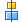
\includegraphics[width=0.7cm]{mActionAlignHCenter} & Центрировать &
 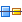
\includegraphics[width=0.7cm]{mActionAlignVCenter} & Центрировать по
 вертикали \\
 \hline 
\includegraphics[width=0.7cm]{mActionAlignTop} & Выровнять по верхним
 краям &
 
\includegraphics[width=0.7cm]{mActionAlignBottom} & Выровнять по нижним
 краям \\
\hline
\end{tabular}
\caption{Инструменты Компоновщика карты}\label{tab:printcomposer_tools}
\end{table}

Все инструменты Компоновщика карты доступны через меню и кнопки на
панели инструментов. Панель инструментов можно скрыть или отобразить
наведя мышку на панель и нажав правую кнопку.

\section{Открытие новой компоновки}\label{composertemplates}

Прежде чем начать работать с компоновкой карты, необходимо загрузить
несколько растровых или векторных слоёв в QGIS и настроить их свойства
удобным для себя образом. После того, как все отрисовывается и выглядит
так, как требуется, нажмите на кнопку
\toolbtntwo{mActionNewComposer}{Создать компоновку карты} на панели
инструментов или выберите \mainmenuopt{Файл} \arrow
\dropmenuopttwo{mActionNewComposer}{Создать компоновку карты}.

\section{Использование компоновщика карт}\label{label_useprintcomposer}

\begin{figure}[ht]
   \centering
   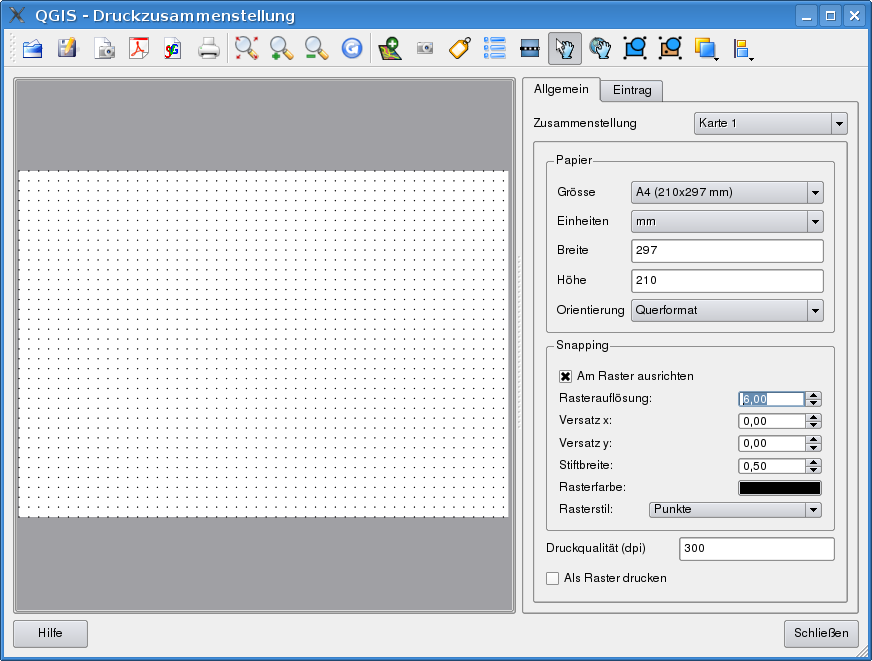
\includegraphics[clip=true, width=\textwidth]{print_composer_blank}
   \caption{Компоновщик Карт \nixcaption}\label{fig:print_composer_blank}
\end{figure}

Открыв компоновку вы увидите пустой лист, на который можно добавить
загруженную в QGIS карту, легенду, масштабную линейку, изображения,
фигуры, стрелки и текст. На рисунке~\ref{fig:print_composer_blank}
показан начальный вид компоновщика с включенным режимом
\checkbox{Прилипать к сетке} но без каких-либо элементов. В окне
компоновщика есть две вкладки:

\begin{itemize}[label=--]
\item на вкладке \tab{Общие} можно настроить размер и ориентацию бумаги,
задать качество печати в dpi и активировать прилипание к сетке с заданным
шагом. Обратите внимание, что функция \checkbox{Прилипать к сетке}
работает только тогда, когда шаг сетки > 0. Здесь же можно активировать
опцию \checkbox{Печатать как растр}. Это значит, что все элементы будут
растеризованы перед печатью или при сохранении в Postscript или PDF.
\item вкладка \tab{Элемент} служит для отображения свойств выделенного
элемента. Для выделения элемента (например, легенды, масштабной линейки
или текста) нажмите кнопку \toolbtntwo{mActionSelectPan}{Выбрать/переместить
элемент}. Затем перейдите на вкладку \tab{Элемент} и настройте свойства
выделенного элемента.
\end{itemize}

На компоновку можно добавить несколько элементов. Так же, в пределах
одной компоновки можно иметь более одной карты, легенды или масштабной
линейки. Каждый элемент имеет свои настройки и, в случае карты, свой
охват.

\section{Добавление карты QGIS на компоновку}

Для добавления карты QGIS, нажмите на кнопку
\toolbtntwo{mActionAddMap}{Добавить карту} в панели инструментов
компоновщика и, зажав левую кнопку мыши, протяните курсор, нарисовав
прямоугольник на листе компоновки. Добавленная карта может отображаться
в одном из трех режимов, выбрать которые можно на вкладке \tab{Элемент}
при выделенной карте:

\begin{itemize}[label=--]
\item \selectstring{{}Предпросмотр}{Прямоугольник} является режимом по
умолчанию. Отображается пустой прямоугольник с текстом
\textit{"Место изображения карты"}.
\item \selectstring{{}Предпросмотр}{Кэш} отрисовывает карту в текущем
разрешении экрана. При выполнении масштабирования в окне компоновщика,
карта не перерисовывается, но само изображение масштабируется.
\item \selectstring{{}Предпросмотр}{Отрисовка} выбор этого режима
означает, что при выполнении масштабирования в окне компоновщика карта
будет перерисовываться, но с целью экономии места только до
максимального разрешения.
\end{itemize}

\textbf{Кэш} является режимом по умолчанию для всех только что
добавленных карт.

Изменить размер карты можно выделив ее при помощи инструмента
\toolbtntwo{mActionSelectPan}{Выбрать/переместить элемент},
и переместив один из голубых маркеров, находящихся в углах. Изменить
другие свойства выделенной карты можно на вкладке \tab{Элемент}.

Для перемещения слоев внутри карты выделите её, затем нажмите на кнопку \\
\toolbtntwo{mActionMoveItemContent}{Переместить содержимое элемента} и
перемещайте слои внутри объекта, зажав левую кнопку мыши.
После того, как элемент расположен в нужном месте, можно зафиксировать
его положение на листе компоновки. Выделите элемент и нажмите правую
кнопку мыши, чтобы \toolbtntwo{mIconLock}{заблокировать} положение
элемента, повторное нажатие разблокирует элемент. Кроме того, можно
заблокировать элементы внутри самой карты активировав настройку
\checkbox{Заблокировать слои для этой карты} в диалоге Карта вкладки
Элемент.

\textbf{Примечание:} QGIS \CURRENT может отображать в компоновке подписи,
созданные новым модулем подписывания, но они некорректно масштабируются.
Поэтому иногда требуется переключаться на стандартный режим подписывания
объектов.

\subsection{Свойства карты "--- диалоги Карта и Границы}

\begin{figure}[ht]
  \centering
  \subfloat[Диалог Карта]{\label{subfig:map_dialog1}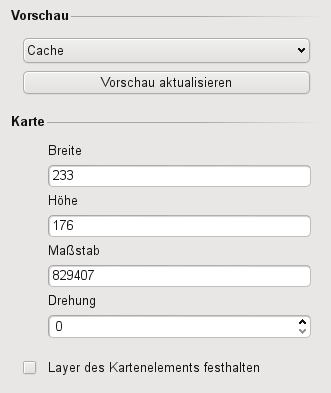
\includegraphics[clip=true, width=0.4\textwidth]{print_composer_map1}}
    \hspace{1cm}
  \subfloat[Диалог Границы]{\label{subfig:map_dialog2}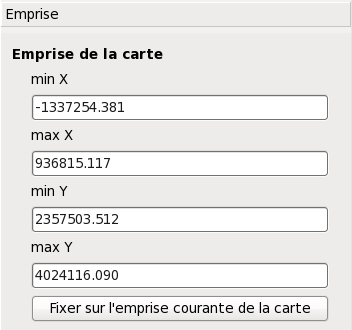
\includegraphics[clip=true, width=0.4\textwidth]{print_composer_map2}}
  \caption{Свойства карты "--- диалоги Карта и Границы \nixcaption}\label{fig:mapdialog}
\end{figure}

\minisec{Диалог Карта}

Диалог \textbf{Карта} состоит из следующих разделов
(см. Рисунок~\ref{fig:mapdialog}a)):

\begin{itemize}[label=--]
\item В разделе \textbf{Предпросмотр} установливаются режимы
предпросмотра Прямоугольник, Кэш и Отрисовка, как описано выше. Для
применения изменений необходимо нажать кнопку \button{Обновить}.
\item В разделе \textbf{Карта} можно изменять размер элемента Карта,
путём редактирования ширины и высоты или масштаба. Поле
\selectstring{{}Вращение}{0} позволяет поворачивать содержимое карты
по часовой стрелке, значения угла задаются в градусах. Обратите
внимение, что фреймы с системой координат по умолчанию добавляются со
значением 0.
\end{itemize}

Если внешний вид карты в главном окне QGIS был изменён в результате
масштабирования или перемещения, либо из-за изменения свойств векторных
или растровых слоёв, обновить карту в окне компоновки можно выделив ее
и нажав на кнопку \button{Обновить}.

\minisec{Диалог Границы}

В диалоге \textbf{Границы} есть разделы:
(смотри Рисунок \ref{fig:mapdialog}b)):

\begin{itemize}[label=--]
\item Раздел \textbf{Границы карты} позволяет указать границы карты,
задавая максимальное и минимальное значения для Y и X или нажав кнопку
\button{Взять с экрана}.
\end{itemize}

Если внешний вид карты в главном окне QGIS был изменён в результате
масштабирования или перемещения, либо из-за изменения свойств векторных
или растровых слоёв, обновить карту в окне компоновки можно выделив ее
и нажав на кнопку \button{Обновить} на вкладке \tab{Элемент} (см.
Рисунок~\ref{fig:mapdialog}a)).

\subsection{Свойства карты "--- диалоги Сетка и Общие параметры}

\begin{figure}[ht]
\centering
   \subfloat[Диалог Сетка]{\label{subfig:map_dialog3}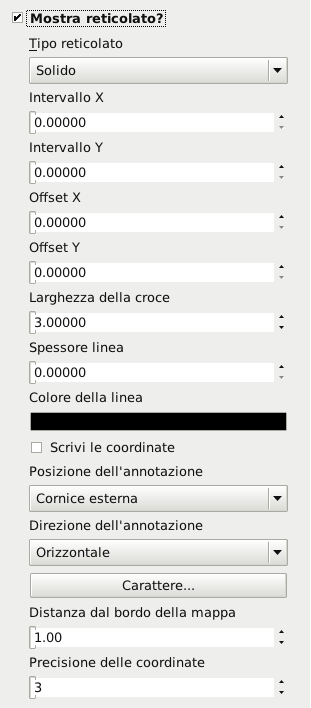
\includegraphics[clip=true, width=0.4\textwidth]{print_composer_map3}}
   \hspace{1cm}
   \subfloat[Диалог Общие параметры]{\label{subfig:map_dialog4}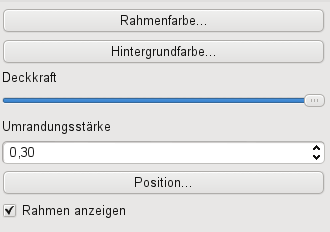
\includegraphics[clip=true, width=0.4\textwidth]{print_composer_map4}}
   \caption{Свойства карты "--- диалоги Сетка и Общие параметры \nixcaption}\label{fig:sec_map_dialog}
\end{figure}

\minisec{Диалог Сетка}

Диалог \textbf{Сетка} предназначен для настройки координатной сетки
(см. Рисунок \ref{fig:sec_map_dialog}a)):

\begin{itemize}[label=--]
\item Флажок \checkbox{Включить сетку?} позволяет наложить сетку на
карту. Сетка может быть в виде линий или в виде перекрестий. Так же
можно задать интервал сетки по X и по Y, смещение по X и по Y, размер
перекрестия или толщину линии.
\item Активация флажка \checkbox{Включить аннотацию} добавит
координаты к рамке карты. Аннотация может выводиться за рамкой карты или
внутри нее. Выводить аннотации можно горизонтально, вертикально,
горизонтально и вертикально или по направлению рамки. И, наконец, можно
задать цвет сетки, шрифт для аннотации, отступ аннотации от рамки и
желаемую точность выводимых координат.
\end{itemize}

\minisec{Диалог Общие параметры}

Диалог \textbf{Общие параметры} используется для настройки внешнего
вида элемента (см. Рисунок~\ref{fig:sec_map_dialog}b)):

\begin{itemize}[label=--]
\item Здесь можно задать цвет и толщину обводки элемента, установить цвет
фона и степень непрозрачности карты. Кнопка \button{Положение} открывает
диалог \dialog{Положение элемента}, где можно задать положение карты
используя точки привязки или координаты. Здесь же можно включить или
выключить отображение рамки элемента при помощи флажка
\checkbox{Включить рамку}.
\end{itemize}

\section{Добавление других элементов к компоновке}

Кроме добавления карты QGIS на компоновку можно добавлять, размещать,
передвигать и настраивать легенду, масштабную линейку, изображения и
текст.

\subsection{Свойства текста "--- диалоги Текст и Общие параметры}

Для добавления текста нажмите на кнопку
\toolbtntwo{mActionLabel}{Добавить текст}, поместите указатель мыши в
нужное место компоновки и нажмите левую кнопку мыши. Изменить свойства
текстового блока можно на вкладке \tab{Элемент}.

\begin{figure}[ht]
\centering
   \subfloat[Диалог Текст]{\label{subfig:labeloptions1}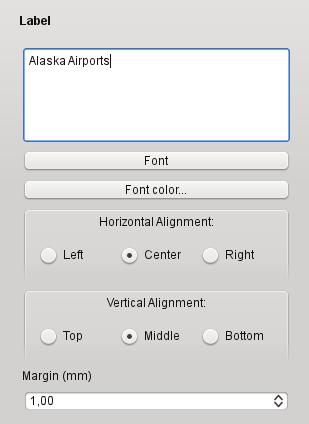
\includegraphics[clip=true, width=0.4\textwidth]{print_composer_label1}}
   \hspace{1cm}
   \subfloat[Диалог Общие параметры]{\label{subfig:labeloptions2}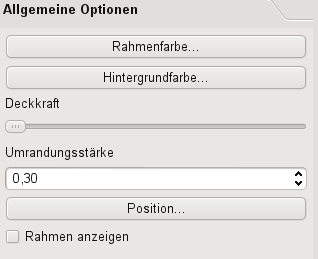
\includegraphics[clip=true, width=0.4\textwidth]{print_composer_label2}}
   \caption{Свойства текста "--- диалоги Текст и Общие параметры \nixcaption}\label{fig:label_option}
\end{figure}

\minisec{Диалог Текст}

Диалог \textbf{Текст} предназначен для управления свойствами текстовых
подписей (см. Рисунок~\ref{fig:label_option}a)):

\begin{itemize}[label=--]
\item диалог \textbf{Текст} позволяет добавить текстовые метки к
компоновке. Здесь можно указать используемый шрифт и его цвет, а также
задать размер полей в мм.
\end{itemize}

\minisec{Диалог Общие параметры}

Диалог \textbf{Общие параметры} поможет вам если надо
(см. Рисунок~\ref{fig:label_option}b)):

\begin{itemize}[label=--]
\item настроить цвет и толщину рамки элемента, задать
цвет фона и степень непрозрачности. Нажатием на кнопку \button{Положение}
вызывается окно \dialog{Положение элемента}, в котором настраивается
положение текста по точкам привязки или по координатам. Здесь же можно
включить или выключить отображение рамки элемента при помощи флажка
\checkbox{Включить рамку}.
\end{itemize}

\subsection{Свойства изображения "--- диалоги Параметры изображения и Общие параметры}

Для добавления изображения нажмите на кнопку
\toolbtntwo{mActionSaveMapAsImage}{Добавить изображение}, поместите
курсор в нужное место компоновки и нажмите левую кнопку мыши, при
необходимости настройте внешний вид на вкладке \tab{Элемент}.

\begin{figure}[ht]
\centering
   \subfloat[Диалог Параметры изображения]{\label{subfig:print_composer_image1}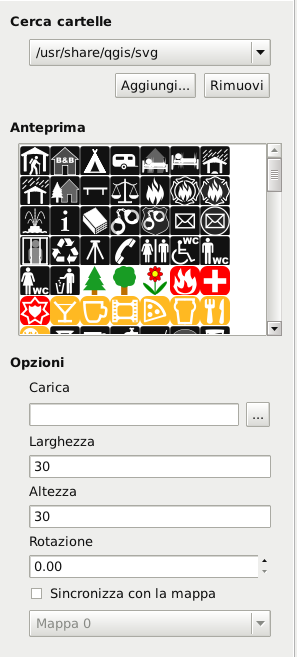
\includegraphics[clip=true, width=0.30\textwidth]{print_composer_image1}}
     \hspace{1cm}
   \subfloat[Диалог Общие параметры]{\label{subfig:print_composer_image2}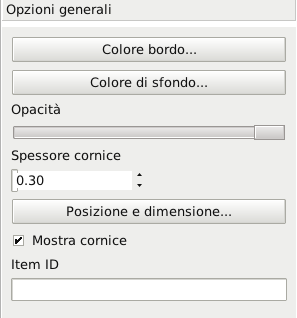
\includegraphics[clip=true, width=0.4\textwidth]{print_composer_image2}}
   \caption{Свойства изображения "--- диалоги Параметры изображения и Общие параметры \nixcaption}\label{fig:imageoptions}
\end{figure}

\minisec{Диалог Параметры изображения}

Диалог \textbf{Параметры изображения} состоит из следующих
разделов (см. Рисунок~\ref{fig:imageoptions}a)):

\begin{itemize}[label=--]
\item В разделе \textbf{Искать в каталогах} добавляются и удаляются
каталоги с изображениями в формате SVG.
\item В поле \textbf{Предпросмотр} показаны все изображения, найденные
в указанных каталогах.
\item Раздел \textbf{Параметры} показывает текущее изображение и
позволяет задать его ширину, высоту и угол поворота по часовой стрелке.
Так же можно указать свой путь к файлам SVG. Установка флажка
\checkbox{Синхронизировать с картой} синхронизирует поворот изображения
на карте QGIS (например, повёрнутый указатель севера) с соответствующим
изображением в компоновке.
\end{itemize}

\minisec{Диалог Общие параметры}

Используя диалог \textbf{Общие параметры} вы можете
(см. Рисунок~\ref{fig:imageoptions}b)):

\begin{itemize}[label=--]
\item настроить цвет и толщину рамки элемента, задать
цвет фона и степень непрозрачности. Нажатием на кнопку \button{Положение}
вызывается диалог \dialog{Положение элемента}, который позволяет
настроить положение изображения, используя точки привязки или координаты.
Здесь же можно включить отображение рамки элемента при помощи флажка
\checkbox{Включить рамку}.
\end{itemize}

\subsection{Свойства легенды "--- диалоги Общие, Элементы легенды и Общие параметры}

Для добавления легенды нажмите кнопку
\toolbtntwo{mActionAddLegend}{Добавить легенду}, поместите указатель
мыши в нужное место компоновки и нажмите левую кнопку мыши. Настроить
внешний вид нового элемента можно на вкладке \tab{Элемент}.

\begin{figure}[h]
\centering
   \subfloat[Диалог Общие]{\label{subfig:print_composer_legend1}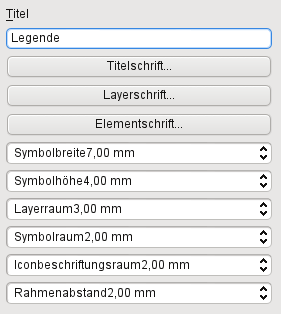
\includegraphics[clip=true, width=0.3\textwidth]{print_composer_legend1}}
   \hspace{1cm}
   \subfloat[Диалог Элементы легенды]{\label{subfig:print_composer_legend2}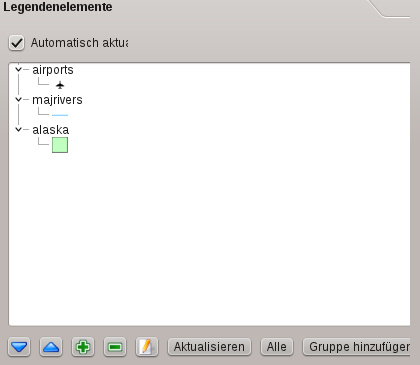
\includegraphics[clip=true, width=0.3\textwidth]{print_composer_legend2}}
   \hspace{1cm}
   \subfloat[Диалог Общие параметры]{\label{subfig:print_composer_legend3}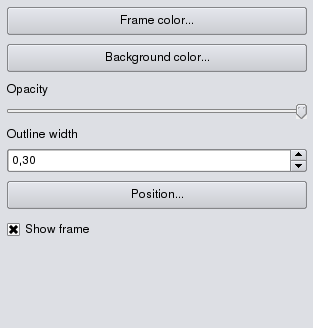
\includegraphics[clip=true, width=0.3\textwidth]{print_composer_legend3}}
   \caption{Свойства легенды "--- диалоги Общие, Элементы легенды и Общие параметры \nixcaption}\label{fig:legendoptions}
\end{figure}

\minisec{Диалог Общие}

Диалог \textbf{Общие} используется для настройки внешнего вида
легенды (см. Рисунок~\ref{fig:legendoptions}a)):

\begin{itemize}[label=--]
\item Здесь можно изменить заголовок легенды. Доступно изменение шрифта
заголовка, группы и слоя. Пользователь может изменять ширину и высоту
знаков, добавлять группы, знаки, подписи и изменять отступы элементов.
\end{itemize}

\minisec{Диалог Элементы легенды}

Вид отдельного элемента легенды настраивается в диалоге
\textbf{Элементы легенды} (см. Рисунок~\ref{fig:legendoptions}b)):

\begin{itemize}[label=--]
\item В этом окне перечисенны все элементы легенды и здесь можно
изменять их порядок, редактировать имена слоев, удалять и восстанавливать
элементы списка. Нажатие на кнопку \button{Update} после изменения
символики в главном окне QGIS, применит эти изменения к элементам
легенды в окне компоновщика. Порядок элементов может быть изменен
кнопками Вверх и Вниз или путём перетаскивания элементов в списке.
\end{itemize}

\minisec{Диалог Общие параметры}

Настройки в диалоге \textbf{Общие параметры} задают общий вид
элемента компоновки (см. Рисунок~\ref{fig:legendoptions}c)):

\begin{itemize}[label=--]
\item Здесь можно настроить цвет и толщину рамки элемента, задать
цвет фона и степень непрозрачности. Нажатием на кнопку
\button{Положение} вызывается диалог \dialog{Положение элемента},
который позволяет настроить положение легенды, используя точки привязки
или координаты. Здесь же можно включить отображение рамки элемента при
помощи флажка \checkbox{Включить рамку}.
\end{itemize}

\subsection{Свойства масштабной линейки "--- диалоги Масштабная линейка и Общие параметры}

Для добавления масштабной линейки нажмите кнопку
\toolbtntwo{mActionAddLegend}{Добавить масштабную линейку}, указатель
мыши в нужное место компоновки и нажмите левую кнопку мыши. Настроить
внешний вид нового элемента можно на вкладке \tab{Элемент}.

\begin{figure}[ht]
\centering
\subfloat[Диалог Масштабная линейка]{\label{subfig:scalebaroptions1}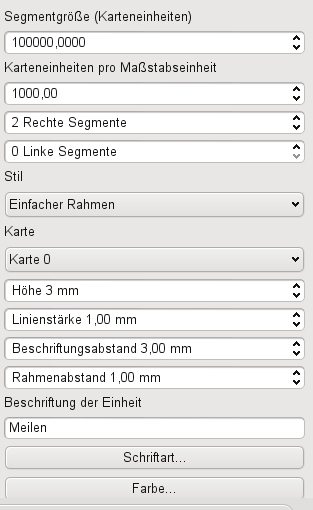
\includegraphics[clip=true, width=0.35\textwidth]{print_composer_scalebar1}}
\hspace{1cm}
\subfloat[Диалог Общие параметры]{\label{subfig:scalebaroptions2}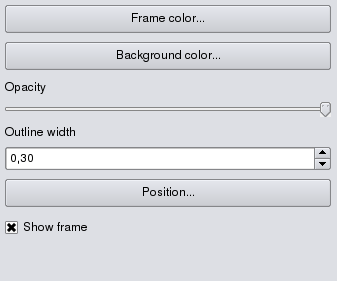
\includegraphics[clip=true, width=0.4\textwidth]{print_composer_scalebar2}}
\caption{Свойства масштабной линейки "--- диалоги Масштабная линейка и Общие параметры \nixcaption}\label{fig:scalebaroptions}
\end{figure}

\minisec{Диалог Масштабная линейка}

Используя диалог \textbf{Масштабная линейка} можно
(см. Рисунок~\ref{fig:scalebaroptions}a)):

\begin{itemize}[label=--]
\item При помощи этого окна можно задать размер сегмента масштабной
линейки в единицах карты, количество единиц карты в одном делении
линейки, и указать сколько сегментов должно отображаться слева и справа
от 0.
\item Установить стиль масштабной линейки. Доступны следующие стили:
одинарная и двойная рамка, штрих вверх-вниз, штрих вверх, штрих вниз и
числовой стиль.
\item Кроме того, можно задать высоту, толщину линии, подпись и отступы
для масштабной линейки. Добавить подпись с единицами измерения, настроить
шрифт и цвет.
\end{itemize}

\minisec{Диалог Общие параметры}

Диалог \textbf{Общие параметры} поможет (см. Рисунок~\ref{fig:scalebaroptions}b)):

\begin{itemize}[label=--]
\item настроить цвет и толщину рамки элемента, задать цвет фона и
степень непрозрачности. Нажатием на кнопку \button{Положение}
вызывается диалог \dialog{Положение элемента}, который позволяет
настроить положение линейки, используя точки привязки или координаты.
Здесь же можно включить отображение рамки элемента при помощи флажка
\checkbox{Включить рамку}.
\end{itemize}

\section{Инструменты навигации}

Для перемещения по компоновке существует 4 основных инструмента:

\begin{itemize}[label=--]
\item \toolbtntwo{mActionZoomIn}{Увеличить},
\item \toolbtntwo{mActionZoomOut}{Уменьшить},
\item \toolbtntwo{mActionZoomFullExtent}{Полный охват} и
\item \toolbtntwo{mActionDraw}{Обновить}, если изображение находится в
несогласованом состоянии.
\end{itemize}

\section{Добавление фигуры и стрелки}

К компоновке можно добавлять фигуры (Эллипс, Прямоугольник, Треугольник)
и стрелки.

\begin{figure}[ht]
\centering
\subfloat[Диалог Фигура]{\label{subfig:shapedialog}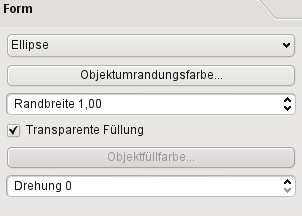
\includegraphics[clip=true, width=0.4\textwidth]{print_composer_shape}}
\hspace{1cm}
\subfloat[Диалог Стрелка]{\label{subfig:arrowdialog}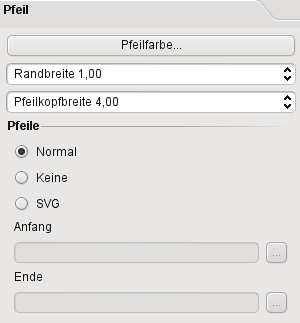
\includegraphics[clip=true, width=0.4\textwidth]{print_composer_arrow}}
\caption{Свойства фигур и стрелок "--- диалоги Фигура и Стрелка \nixcaption}\label{fig:shapearrow}
\end{figure}

\begin{itemize}[label=--]
\item Диалог \textbf{Фигура} позволяет нарисовать на компоновке эллипс,
прямоугольник или треугольник. Можно настроить цвет обводки и заливки,
толщину обводки и угол поворота по часовой стрелке.
\item Диалог \textbf{Стрелка} предназначен для рисования стрелок на
компоновке. Доступна настройка цвета, толщины линии и размера маркера.
Есть возможность использовать маркер по умолчанию, отказаться от маркера
или загрузить его из файла SVG. При использовании маркеров в формате SVG
можно задать отдельно маркер конца и маркер начала.
\end{itemize}

\section{Добавление значений из таблицы атрибутов}

Возможно добавление на компоновку части атрибутивной таблицы векторного
слоя.

\begin{figure}[ht]
\centering
\subfloat[Диалог Таблица]{\label{subfig:tabledialog1}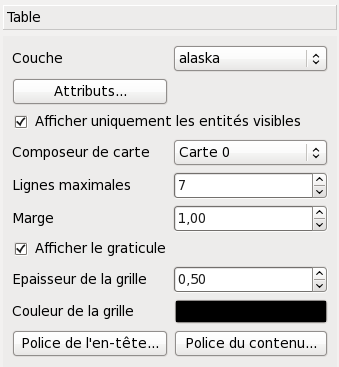
\includegraphics[clip=true, width=0.38\textwidth]{print_composer_attribute1}}
\hspace{1cm}
\subfloat[Диалог Общие параметры]{\label{subfig:tabledialog2}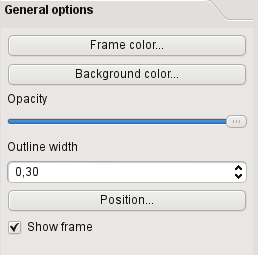
\includegraphics[clip=true, width=0.38\textwidth]{print_composer_attribute2}}
\caption{Свойства таблицы атрибутов "--- диалоги Таблица и Общие параметры \nixcaption}\label{fig:attrcomp}
\end{figure}

\minisec{Диалог Таблица}

Диалог \textbf{Таблица} предоставляет следующий функционал
(см. Рисунок~\ref{fig:attrcomp}a)):

\begin{itemize}[label=--]
\item В диалоге \textbf{Таблица} выбирается векторный слой и столбцы
атрибутивной таблицы. Можно указать максимальное количество видимых
записей или включить отображение атрибутов только видимых на компоновке
объектов. Есть возможность настроить отображение сетки таблицы и задать
шрифт для заголовков и содержимого.
\end{itemize}

\minisec{Диалог Общие параметры}

Диалог \textbf{Общие параметры} используется, когда необходимо
(см. Рисунок~\ref{fig:attrcomp}b)):

\begin{itemize}[label=--]
\item настроить цвет и толщину рамки элемента, задать
цвет фона и степень непрозрачности. Нажатием на кнопку \button{Положение}
вызывается диалог \dialog{Положение элемента}, который позволяет
настроить положение таблицы, используя точки привязки или координаты.
Здесь же можно включить отображение рамки элемента при помощи флажка
\checkbox{Включить рамку}.
\end{itemize}

\section{Сортировка и выравнивание элементов}

Функции сортировки элементов находятся в выпадающем меню
\toolbtntwo{mActionRaiseItems}{Поднять выбранные элементы}. Выделите
элемент компоновки и выберите необходимое действие чтобы расположить
выделенный элемент выше или ниже других (см. таблицу~\ref{tab:printcomposer_tools}).

Инструменты выравнивания доступны через выпадающее меню \\
\toolbtntwo{mActionAlignLeft}{Выровнять выбранные элементы по левым краям}
(см. таблицу~\ref{tab:printcomposer_tools}). Перед использованием
инструмента выравнивания необходимо выделить несколько элементов, а
затем нажать кнопку соответствующего инструмента. Все выделенные объекты
будут выровнены в пределах их общих границ.

\section{Создание вывода}

На Рисунке~\ref{fig:print_composer_complete} показан пример компоновки,
которая содержит все вышеописанные элементы.

\begin{figure}[h]
   \centering
   \includegraphics[clip=true, width=\textwidth]{print_composer_complete}
   \caption{Компоновка с добавленными картой, легендой, масштабной линейкой, координатами и текстом \nixcaption} \label{fig:print_composer_complete}
\end{figure}

Компоновщик печати позволяет экспортировать результат в несколько
форматов, при этом можно задавать разрешение (качество печати) и размер
бумаги:

\begin{itemize}[label=--]
\item Кнопка \toolbtntwo{mActionFilePrint}{Печать} предназначена для
печати компоновки на подключенный принтер или в Postscript файл, в
зависимости от установленных драйверов принтера.
\item Нажатием на кнопку
\toolbtntwo{mActionExportMapServer}{Экспорт в изображение}
компоновку можно экспортировать в один из графических форматов: PNG,
BPM, TIF, JPG\dots
\item Нажав на кнопку \toolbtntwo{mActionSaveAsPDF}{Экспорт в PDF} вы
сохраните компоновку в формате PDF.
\item Кнопка \toolbtntwo{mActionSaveAsSVG}{Экспорт в SVG} создаст из
компоновки файл формата SVG (Scalable Vector Graphic).
\textbf{Примечание:} Сейчас сохранение в SVG работает на базовом уровне.
Это не проблема QGIS, а недостаток нижележащих библиотек Qt. Вероятно,
в будущем эти проблемы будут решены.
\end{itemize}

\section{Сохранение и загрузка шаблона}

При помощи кнопок \toolbtntwo{mActionFileSaveAs}{Сохранить как шаблон}
и \toolbtntwo{mActionFolder}{Загрузить из шаблона} состояние открытой
компоновки можно сохранить как *.qpt шаблон и загрузить шаблон в другой
сессии.

Кнопка \toolbtntwo{mActionComposerManager}{Управление компоновками}
на панели инструментов и пункт меню \\
\mainmenuopt{Файл} \arrow \dropmenuopttwo{mActionComposerManager}{Управление компоновками}
позволяют добавлять новые и управлять существующими компоновками.

\begin{figure}[h]
   \centering
   \includegraphics[clip=true, width=8cm]{print_composer_manager}
   \caption{Управление компоновками \nixcaption}
   \label{fig:print_composer_manager}
\end{figure}

\FloatBarrier
